%!TEX program = xelatex

\documentclass{ctexart}
    \usepackage{amsmath}
    \usepackage{pgf}
    \usepackage{tikz}
    \usetikzlibrary{arrows,automata}
    % \usepackage[latin1]{inputenc}
    \usepackage{verbatim}
    \title{Solution for Homework1}
    \author{徐翔哲(161250170)} 
    
\begin{document}
\maketitle
\newpage
% 1-1-1
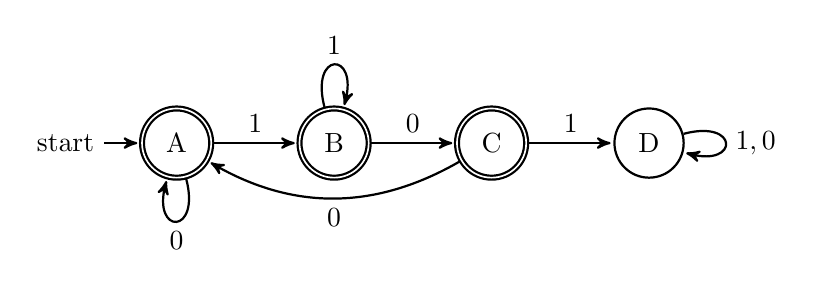
\begin{tikzpicture}
	[->,>=stealth',shorten >=1pt,auto,node distance=2cm,
		thick,base node/.style={circle,draw,minimum size=16pt}, real node/.style={double,circle,draw,minimum size=35pt}]


    \node[initial, initial text={start},accepting, state] (A) {A};
    \node[accepting, state] (B)[right of = A] {B};
    \node[accepting, state] (C)[right of = B] {C};
    \node[state] (D)[right of = C] {D};

	% \node[initial,initial text={}, accepting, state] (1) {$\epsilon$};
	% \node[state](2)[right of=1 ]{$51$}[above];

	\path[]
    (A) edge [loop below]   node {$0$}  (A)
        edge                node {$1$}     (B)
    (B) edge [loop above]   node {$1$}  (B)
        edge                node {$0$}  (C)
    (C) edge [bend left]   node {$0$}  (A)
        edge                node {$1$}  (D)
    (D) edge [loop right]   node {$1,0$} (D)
    ;


\end{tikzpicture}
% 1-1-2
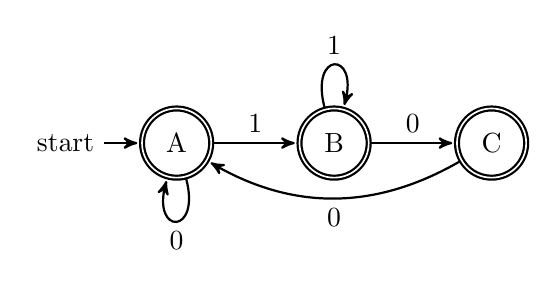
\begin{tikzpicture}
    [->,>=stealth',shorten >=1pt,auto,node distance=2cm,
        thick,base node/.style={circle,draw,minimum size=16pt}, real node/.style={double,circle,draw,minimum size=35pt}]
        

    \node[initial, initial text={start},accepting, state] (A) {A};
    \node[accepting, state] (B)[right of = A] {B};
    \node[accepting, state] (C)[right of = B] {C};

    \path[]
    (A) edge [loop below]   node {$0$}  (A)
        edge                node {$1$}     (B)
    (B) edge [loop above]   node {$1$}  (B)
        edge                node {$0$}  (C)
    (C) edge [bend left]   node {$0$}  (A)
    ;
\end{tikzpicture}
% branch1-1
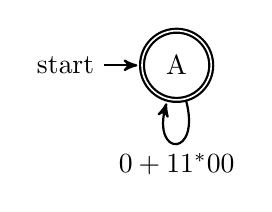
\begin{tikzpicture}
    [->,>=stealth',shorten >=1pt,auto,node distance=2cm,
        thick,base node/.style={circle,draw,minimum size=16pt}, real node/.style={double,circle,draw,minimum size=35pt}]
        

    \node[initial, initial text={start},accepting, state] (A) {A};

    \path[]
    (A) edge [loop below]   node {$0+11^*00$}  (A)
        % edge                node {$1$}     (B)
    % (B) edge [loop above]   node {$1$}  (B)
    %     edge                node {$0$}  (C)
    % (C) edge [bend left]   node {$0$}  (A)
    ;
\end{tikzpicture}
% branch 1-2
\begin{tikzpicture}
    [->,>=stealth',shorten >=1pt,auto,node distance=2cm,
        thick,base node/.style={circle,draw,minimum size=16pt}, real node/.style={double,circle,draw,minimum size=35pt}]
        

    \node[initial, initial text={start},accepting, state] (A) {A};
    \node[accepting, state] (C)[right of = B] {C};

    \path[]
    (A) edge [loop below]   node {$0$}  (A)
        edge                node {$11^*0$}     (C)
    (C) edge [bend left]   node {$0$}  (A)
    ;
\end{tikzpicture}
% branch 2
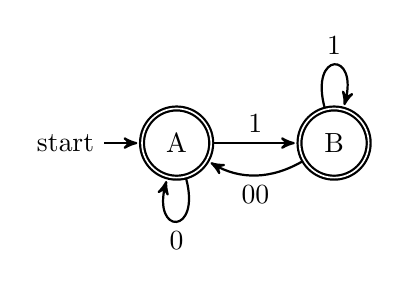
\begin{tikzpicture}
    [->,>=stealth',shorten >=1pt,auto,node distance=2cm,
        thick,base node/.style={circle,draw,minimum size=16pt}, real node/.style={double,circle,draw,minimum size=35pt}]
        

    \node[initial, initial text={start},accepting, state] (A) {A};
    \node[accepting, state] (B)[right of = A] {B};

    \path[]
    (A) edge [loop below]   node {$0$}  (A)
        edge                node {$1$}     (B)
    (B) edge [loop above]   node {$1$}  (B)
        edge [bend left]    node {$00$}  (A)
    ;
\end{tikzpicture}

\end{document}